\documentclass[11pt]{article}
\usepackage[margin=1in]{geometry}
\usepackage{amsmath,amssymb,amsthm}
\usepackage{graphicx}
\usepackage{booktabs}
\usepackage{tabularx}
\usepackage[authoryear,round]{natbib}
\usepackage{algorithm}
\usepackage{algpseudocode}
\usepackage{tikz}
\usetikzlibrary{arrows.meta,shapes.geometric}
\usepackage{xcolor}
\usepackage{caption}
\usepackage{microtype}
\usepackage{url}
\usepackage[hidelinks]{hyperref}

\definecolor{accent}{HTML}{2A78D6}
\definecolor{quiet}{HTML}{52514E}
\definecolor{edge}{HTML}{A8A69E}

\newtheorem{proposition}{Proposition}
\newcommand{\A}{\mathcal{A}}
\newcommand{\KL}{\mathrm{KL}}
\newcommand{\Unif}{U}
\newcommand{\E}{\mathbb{E}}
\DeclareMathOperator{\JS}{JS}
\captionsetup{font=small,labelfont=bf}

\title{Online Stochastic Trial Minimisation}
\author{Andrew Bistras\thanks{Correspondence: \href{mailto:andrew.bistras@gmail.com}{andrew.bistras@gmail.com}. Code, simulations and this manuscript: \url{https://github.com/andrewbistras/min_sim}.}\\[4pt]
{\normalsize University of California, Los Angeles}\\
{\normalsize Astrid Cybernetics}}
\date{Draft, October 17, 2026}

\begin{document}
\maketitle

\begin{abstract}
\noindent Human subjects research often gives each participant a set of conditions from a larger pool, such as vignettes, choice sets, intervention components or treatment sequences. Investigators want every condition used equally often at every point of enrollment. Complete randomization balances exposure only in expectation, and least-filled quotas are deterministic, so they fail when participants enroll at the same time or drop out unevenly. We generalize minimisation, the balancing method of clinical trials, to sets of conditions under within-participant constraints, and show that it is a feedback controller with one natural parameter: the bits of randomness each allocation may give up. The algorithm rolls one weighted die whose faces are the conditions, reweighs the faces after every participant, and keeps a roll only when it forms an admissible set. The temperature is solved so that each allocation spends exactly its budget. The rule is the maximum-entropy allocation for its expected balance, and its balance criterion is a second-order Jensen--Shannon divergence between the allocation history and the new allocation. A fixed-temperature version solves an entropy-regularized control problem exactly, and imbalance stays bounded. In simulations of a $2^6$ vignette design with five vignettes per participant and no minimal pairs, a budget of 1 bit (of 28.3 available) kept the exposure SD near 0.9 over 1,000 participants, against 8.4 under complete randomization. It stayed stable when 64 participants shared a stale ledger, where deterministic minimisation did three times worse than randomization, and with a ledger of completions it corrected the unequal condition representation caused by differential attrition.
\end{abstract}

\noindent\textbf{Keywords:} minimisation; adaptive randomization; counterbalancing; vignette studies; entropy; online enrollment; attrition.

%======================================================================
\section{Introduction}

Human subjects research often gives each participant several conditions drawn from a larger set, and investigators want every condition used about equally often. The pattern runs across fields: case vignettes rated by clinicians or the public \citep{peabody2000,auspurg2015}, discrete choice experiments in health economics \citep{johnson2013}, crossover trials \citep{senn2002}, and factorial experiments that screen intervention components \citep{collins2018}. Our running example is a vignette study in which six binary attributes define 64 vignettes and each participant rates five.

\paragraph{Complete randomization balances exposure only in expectation.} With 64 vignettes and five per participant, the counts after 320 participants scatter with a standard deviation of about 4.6 around a target of 25. The most- and least-shown vignettes then differ by about 21 showings, so precision varies across stimuli, and a study that stops early or loses data to exclusions can leave some vignettes nearly unobserved.

\paragraph{Enrollment is sequential, bursty and leaky, and quota tools handle it badly.} Participants arrive one at a time, often at several sites or through several recruitment channels at once, and some leave before they finish. Common tools allocate the least-filled conditions, such as Qualtrics' ``evenly present elements,'' Gorilla's counterbalancing nodes and psiTurk's choice among the least-filled conditions \citep{gureckis2016}; apart from tie-breaking these rules are deterministic, so simultaneous enrollments receive the same allocation. Counts of assignments rather than completions also drift when dropout differs by condition, as it often does \citep{zhou2016,bell2013}.

\paragraph{Constraints within a participant make the problem harder.} Researchers often forbid ``minimal pairs'' (two vignettes that differ in one factor only) because such pairs expose the manipulation and invite demand effects \citep{charness2012,horiuchi2022}. The evidence that demand effects are large is mixed \citep{mummolo2019,clifford2021}, so the rule is cheap insurance rather than a necessity. Either way, the least-filled stimuli may be mutually incompatible, and quota rules have no principled way to trade balance against the constraint.

\paragraph{Clinical trials met a version of this problem fifty years ago.} Minimisation assigns each new participant to the arm that most reduces imbalance \citep{taves1974,pocock1975,altman2005}. It appears in roughly one in ten trials published in leading medical journals \citep{kahan2012,ciolino2019}, and regulators accept it when each allocation keeps a random element \citep{ich1998,ema2015}. A long literature asks how much randomness to keep, from Efron's biased coin \citep{efron1971} and Klotz's maximum-entropy allocation \citep{klotz1978} to modern comparisons of balance and predictability \citep{atkinson2014}.

\paragraph{Those methods allocate one treatment per participant.} None of them handles constrained sets of conditions, simultaneous enrollment or the unequal condition counts that differential attrition leaves. Minimisation over the 16 cells of a $2^4$ factorial trial made 34\% of allocations deterministic \citep{kuhn2019}, social scientists have minimized over respondents' covariates \citep{moore2013}, and adaptive vignette allocation has been limited to a biased coin on a single factor \citep{kim2024}.

\paragraph{This paper generalizes minimisation to allocating sets of conditions as participants enroll, treating it as a feedback controller with one reportable parameter.} That parameter is the number of bits of randomness each participant's allocation may give up. The algorithm keeps one weighted die whose faces are the conditions, reweighs the faces after every participant, and rolls it until the faces form an admissible set. The contributions are:
\begin{enumerate}
\item A framing of allocation as feedback control, which explains why the controller must stay random when participants enroll at the same time.
\item An exact, simple algorithm whose single parameter has a direct reading: a budget of $\kappa$ bits leaves each allocation as random as a uniform draw from a fraction $2^{-\kappa}$ of all admissible sets, and caps at $\kappa$ bits what anyone who knows the history can learn about the next allocation.
\item Theory linking the method to maximum entropy, the Jensen--Shannon divergence and entropy-regularized optimal control, with a stability guarantee.
\item Simulations of a 64-vignette design covering balance, simultaneous enrollment, differential attrition and order effects; a JavaScript implementation; and guidance for protocols and reports.
\end{enumerate}

%======================================================================
\section{The allocation problem}\label{sec:problem}

Each participant receives a deck of $k$ stimuli from a pool of $m$, and we want the running exposure counts to stay equal while every deck stays random.

\paragraph{Setting.} Participants arrive one at a time, or in bursts. Participant $t$ receives a deck $S_t$: a set of $k$ distinct stimuli, shown in some order. A compatibility rule between pairs of stimuli defines the admissible decks, written $\A$.

\paragraph{The ledger.} Let $c_i(t)$ be the number of the first $t$ decks that contain stimulus $i$. With equal targets, each stimulus should have been shown $kt/m$ times after $t$ participants. The ledger is the only state the allocator needs.

\paragraph{Running example.} Six binary factors define $m=64$ vignettes, each coded as a 6-bit string. Each participant rates $k=5$ of them, and no two vignettes in a deck may differ in exactly one factor (Hamming distance at least 2). In graph terms, admissible decks are independent sets of size five in the six-dimensional hypercube.

\paragraph{How much room the constraint leaves.} Of the 7,624,512 five-vignette sets, 2,682,432 (35.2\%) are admissible. With 120 presentation orders each, that gives 321,891,840 ordered decks, or 28.26 bits: the most randomness any single allocation can carry. The order supplies 6.91 of those bits; the choice of set supplies the other 21.36.

\paragraph{Complete randomization is balanced only in expectation.} Every vignette has the same six forbidden partners, so a uniform draw from $\A$ includes each vignette with probability exactly $5/64$. The problem is the fluctuation around that expectation, which grows with the square root of the number of participants.

\begin{table}[ht]
\centering\small
\caption{What a good allocator delivers.}\label{tab:goals}
\begin{tabularx}{\textwidth}{@{}lXl@{}}
\toprule
Goal & Measure & Ideal \\
\midrule
Balanced exposure at every point & SD of $c_i(t)$ around $kt/m$; range of the counts & as small as integer counts allow \\
A random allocation for each participant & Entropy $H_t$ of the allocation law, in bits & close to the 28.26-bit maximum \\
Robustness online & Balance when $b$ participants share one stale ledger; balance among completers when dropout differs & unaffected \\
No order effects by design & Presentation order & uniform over the 120 orders \\
\bottomrule
\end{tabularx}
\end{table}

\paragraph{Bits spent.} We measure how far an allocation departs from complete randomization by the bits it gives up,
\begin{equation}\label{eq:kappa}
\kappa_t \;=\; \log_2|\A| - H(\pi_t) \;=\; \KL\big(\pi_t \,\big\|\, \Unif\big),
\end{equation}
where $\pi_t$ is the probability distribution over admissible sets used for participant $t$ and $\Unif$ is the uniform distribution on $\A$. A budget of $\kappa$ bits leaves the allocation as random as a uniform choice among a fraction $2^{-\kappa}$ of the admissible decks: 1 bit means half of them, 2 bits a quarter.

\paragraph{Exposure imbalance.} We summarize balance by the standard deviation of the counts around their target,
\begin{equation}
\operatorname{sd}(t) \;=\; \Big(\frac{1}{m}\sum_{i=1}^{m}\big(c_i(t) - kt/m\big)^{2}\Big)^{1/2}.
\end{equation}
Under complete randomization $\operatorname{sd}(t)$ grows like $\sqrt{t}$. A good minimisation rule keeps it bounded for all $t$.

%======================================================================
\section{Minimisation as feedback control}\label{sec:control}

Allocation is a control problem: the ledger accumulates every decision, and the allocator steers it back toward equal exposure.

\paragraph{The ledger integrates the allocations.} Write $e_i(t) = c_i(t) - kt/m$ for stimulus $i$'s surplus over its target. Each deck adds one showing to each of its stimuli and raises every target by $k/m$, so with $x(S)$ the 0/1 inclusion vector of deck $S$,
\begin{equation}
e(t+1) \;=\; e(t) + x(S_t) - \tfrac{k}{m}\mathbf{1}.
\end{equation}
Under complete randomization $e(t)$ is a random walk and drifts away like $\sqrt{t}$. Any rule that looks at $e(t)$ before choosing $S_t$ is a feedback controller for this integrator.

\paragraph{Open loop or closed loop.} A schedule of decks fixed in advance, such as a Latin square or an offline D-efficient design, is open-loop control. It is exact only if every participant completes, in order, and the study stops where planned. Online, participants drop out, arrive in bursts, and studies are stopped early or extended, so the allocator has to read the ledger and correct what actually happened.

\paragraph{Deterministic minimisation is the high-gain limit.} Because every deck has the same number of stimuli, the squared surplus after deck $S$ differs between decks only through the counts of its members:
\begin{equation}
\big\| e + x(S) - \tfrac{k}{m}\mathbf{1}\big\|^{2} \;=\; \|e\|^{2} + 2\sum_{i\in S} c_i + \text{const}.
\end{equation}
Minimizing it means choosing the admissible deck with the smallest total count. This is Taves's (\citeyear{taves1974}) minimisation applied to decks; in machine learning the same rule is called herding \citep{welling2009}.

\paragraph{Weakness 1: delay.} When participants arrive faster than the ledger updates, several of them see the same counts, and a deterministic rule hands them all the same least-shown stimuli. A high-gain controller with a delay in its loop overshoots; Section~\ref{sec:sims} measures how badly.

\paragraph{Weakness 2: predictability.} Anyone who knows the counts can foresee a deterministic allocation. In trials that lets recruiters steer which participant receives which condition, the selection bias that allocation concealment exists to prevent \citep{blackwell1957,schulz2002}. It also leaves randomization-based inference nothing to work with, and its pattern can line up with drifts in who enrolls when.

\paragraph{Stochastic minimisation softens the rule.} We choose each admissible deck with probability
\begin{equation}\label{eq:gibbs}
\pi_\beta(S) \;=\; \frac{\exp\big(-\beta\sum_{i\in S} c_i\big)}{\sum_{S'\in\A}\exp\big(-\beta\sum_{i\in S'} c_i\big)}, \qquad S\in\A.
\end{equation}
Setting $\beta=0$ gives complete randomization; letting $\beta$ grow without bound gives deterministic minimisation with random tie-breaking. In control terms $\beta$ is the gain of the feedback; in statistical physics $1/\beta$ is a temperature.

\paragraph{The single parameter is entropy, not gain.} A given $\beta$ is gentle when the counts are nearly equal and forceful when they are far apart, so it has no fixed meaning. We let the researcher fix the bits each allocation may give up, $\kappa$, and solve for $\beta$ participant by participant:
\begin{equation}\label{eq:budget}
\KL\big(\pi_{\beta_t}\,\big\|\,\Unif\big) \;=\; \kappa \quad\text{for every participant } t.
\end{equation}
The budget means the same thing in every design and at every point in a study, which is what a single default needs.

\begin{figure}[t]
\centering
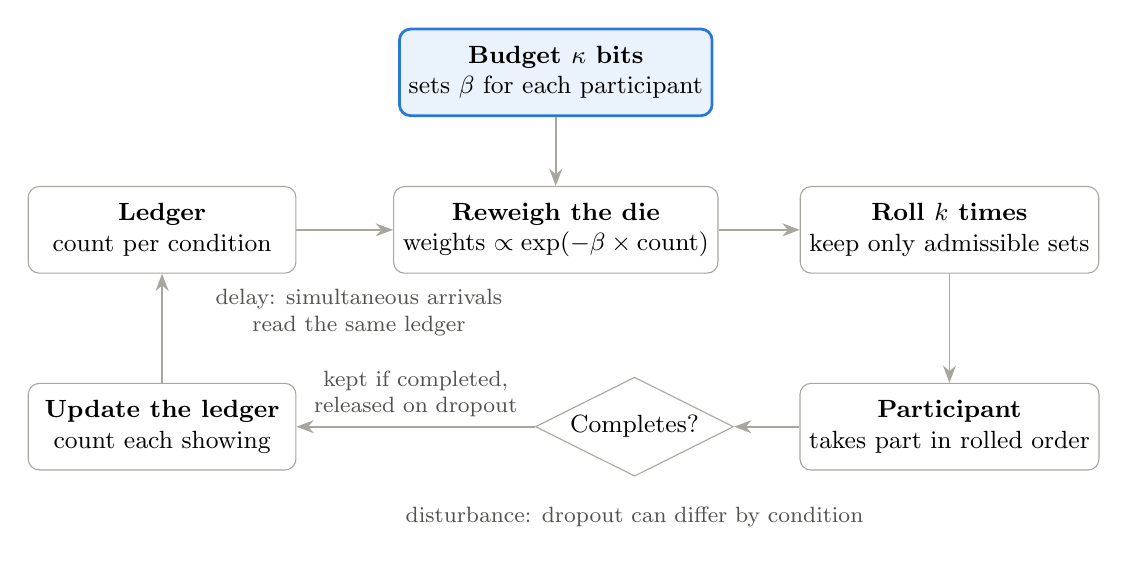
\begin{tikzpicture}[
  box/.style={draw=edge, rounded corners=4pt, minimum width=3.4cm, minimum height=1.1cm, align=center, font=\small},
  arr/.style={-{Stealth[length=2.2mm]}, draw=edge, line width=0.6pt},
  note/.style={font=\footnotesize, text=quiet, align=center}]
\node[box, draw=accent, line width=1pt, fill=accent!10] (budget) at (0,2.0) {\textbf{Budget $\kappa$ bits}\\ sets $\beta$ for each participant};
\node[box] (ledger) at (-5.0,0) {\textbf{Ledger}\\ count per condition};
\node[box] (reweigh) at (0,0) {\textbf{Reweigh the die}\\ weights $\propto \exp(-\beta\times\mathrm{count})$};
\node[box] (roll) at (5.0,0) {\textbf{Roll $k$ times}\\ keep only admissible sets};
\node[box] (participant) at (5.0,-2.5) {\textbf{Participant}\\ takes part in rolled order};
\node[draw=edge, diamond, aspect=2, inner sep=1.5pt, font=\small] (completes) at (1.0,-2.5) {Completes?};
\node[box] (update) at (-5.0,-2.5) {\textbf{Update the ledger}\\ count each showing};
\draw[arr] (budget) -- (reweigh);
\draw[arr] (ledger) -- (reweigh);
\draw[arr] (reweigh) -- (roll);
\draw[arr] (roll) -- (participant);
\draw[arr] (participant) -- (completes);
\draw[arr] (completes) -- node[note, above]{kept if completed,\\ released on dropout} (update);
\draw[arr] (update) -- (ledger);
\node[note] at (-2.5,-1.05) {delay: simultaneous arrivals\\ read the same ledger};
\node[note] at (1.0,-3.65) {disturbance: dropout can differ by condition};
\end{tikzpicture}
\caption{Allocation is a feedback loop, and only completed sessions keep their count. The budget is the only setting; the ledger, the die and the admissibility rule are fixed by the design.}\label{fig:loop}
\end{figure}

%======================================================================
\section{The algorithm: reweighted dice}\label{sec:algorithm}

The allocation law factorizes over the deck's members, so it can be sampled exactly by rolling one weighted die $k$ times and keeping only admissible rolls.

\paragraph{Why dice.} The weight of a deck is a product over its members,
\[
\exp\Big(-\beta\sum_{i\in S}c_i\Big) \;=\; \prod_{i\in S}\exp(-\beta c_i).
\]
Roll $k$ times a die whose face $i$ has probability proportional to $\exp(-\beta c_i)$, keep the roll when its faces form an admissible deck, and the kept decks follow $\pi_\beta$ exactly (Proposition~\ref{prop:dice}). Because the same die is rolled for every slot, the presentation order is a uniformly random shuffle at no extra cost.

\paragraph{Reweighing after every participant.} The die's weights are recomputed from the ledger before each allocation, and each showing divides a face's weight by $e^{\beta}$. Faces shown less often become heavier until the counts even out, and the solved temperature keeps each reweighing within the budget.

\begin{algorithm}[t]
\caption{Online stochastic trial minimisation, one allocation}\label{alg:ostm}
\begin{algorithmic}[1]
\Require ledger $c\in\mathbb{N}^m$, admissible sets $\A$, deck size $k$, budget $\kappa$ bits
\State $d_i \gets c_i - \min_j c_j$ for $i = 1,\dots,m$
\State find $\beta \ge 0$ with $\KL(\pi_\beta \,\|\, \Unif) = \kappa\ln 2$; if ties among the least-shown decks leave less to gain, set $\beta \gets \infty$
\State $w_i \gets \exp(-\beta d_i)$ for $i = 1,\dots,m$ \Comment{reweigh the die}
\Repeat
  \State roll $s_1,\dots,s_k$ independently with $\Pr(s_p = i) \propto w_i$
\Until{$s_1,\dots,s_k$ are distinct and pairwise compatible}
\State present the conditions in the order $s_1,\dots,s_k$
\State log the set, $\beta$ and $\log \pi_\beta(\{s_1,\dots,s_k\})$
\State update the ledger (Section~\ref{sec:recs} discusses when a participant should count)
\end{algorithmic}
\end{algorithm}

\paragraph{Calibrating $\beta$ exactly.} For designs of moderate size we enumerate $\A$ once: 2,682,432 sets in the example, in 107 ms. For each participant we tally $N_E$, the number of admissible decks whose offsets sum to $E = \sum_{i\in S} d_i$. The information spent is then a function of $\beta$ alone (in nats; divide by $\ln 2$ for bits):
\begin{equation}\label{eq:calib}
\kappa(\beta) \;=\; \log|\A| - \log\sum_E N_E\,e^{-\beta E} - \beta\,\bar E_\beta,
\qquad \bar E_\beta \;=\; \frac{\sum_E E\,N_E\,e^{-\beta E}}{\sum_E N_E\,e^{-\beta E}}.
\end{equation}
$\kappa(\beta)$ rises monotonically from 0 to $\log(|\A|/N_{E_{\min}})$, so bisection finds $\beta$ to machine precision. One allocation, calibration included, takes 8--10 ms in Node.js, and about 18 ms at the very start of a study, when every deck ties.

\paragraph{Larger designs.} When $\A$ is too large to enumerate, $\kappa(\beta)$ can be estimated from the dice themselves. With $\tilde w$ the die's normalized weights and $A(\beta)$ the probability that $k$ rolls are admissible,
\begin{equation}
\KL(\pi_\beta\,\|\,\Unif) \;=\; \E_{\pi_\beta}\Big[\sum_{p=1}^{k}\log\big(m\,\tilde w_{s_p}\big)\Big] - \log\frac{A(\beta)}{A(0)}.
\end{equation}
Reusing the same random numbers across candidate values of $\beta$ keeps the estimate smooth enough for bisection.

\paragraph{How many rolls.} Under complete randomization 30\% of rolls are admissible, and at budgets up to 2 bits the rate stayed between 24\% and 31\%, so a deck takes three or four rolls. At 4 bits it occasionally fell to 2\% (about 50 rolls), when the die piled onto a few least-shown faces. If rolling keeps failing, the implementation draws directly from the enumerated list, which it also does whenever $\beta=\infty$.

\paragraph{Using the implementation.} The JavaScript module has no dependencies and runs in Node.js or a browser:
\begin{verbatim}
import { hypercubeConflicts, createDesign, createAllocator } from './ostm.js';
const design = createDesign({ ...hypercubeConflicts(6, 2), k: 5 });
const allocator = createAllocator(design, { budgetBits: 1 });
const { deck, logProbSet } = allocator.allocate(counts);  // counts = the ledger
\end{verbatim}
Each call returns the deck in presentation order and the log probability of its set of stimuli, for the analysis log.

%======================================================================
\section{Theory}\label{sec:theory}

Five results explain why the reweighted die is the right object: it is the maximum-entropy rule, it samples exactly, it maximizes a Jensen--Shannon gain, it solves an optimal-control problem exactly, and it keeps imbalance bounded. Throughout, $E(S) = \sum_{i\in S}c_i$ and $\Unif$ is the uniform law on $\A$. Proofs are in Appendix~\ref{app:proofs}.

\begin{proposition}[Maximum entropy]\label{prop:maxent}
Let $\beta>0$. Every law $\pi$ on $\A$ with $\KL(\pi\,\|\,\Unif)\le\KL(\pi_\beta\,\|\,\Unif)$ has $\E_\pi[E]\ge\E_{\pi_\beta}[E]$. Equivalently, among laws with the same expected total count, $\pi_\beta$ has the most entropy.
\end{proposition}
This is Jaynes's (\citeyear{jaynes1957}) maximum-entropy principle, which \citet{klotz1978} applied to allocating single treatments.

\begin{proposition}[Exact dice]\label{prop:dice}
Let $s_1,\dots,s_k$ be independent with $\Pr(s_p=i)\propto e^{-\beta c_i}$. Conditional on $\{s_1,\dots,s_k\}$ being an admissible set, the set has law $\pi_\beta$ and its $k!$ orders are equally likely. The acceptance probability is $k!\sum_{S\in\A}\prod_{i\in S}\tilde w_i$.
\end{proposition}

\begin{proposition}[Jensen--Shannon identity]\label{prop:js}
Let $P_t(i)=c_i(t)/(kt)$ be the ledger's distribution of showings, $U_S$ the uniform distribution on the members of $S$, and $w=t/(t+1)$, so that adding $S$ gives $P_{t+1}=wP_t+(1-w)U_S$ and
\[
\JS_w(P_t,U_S) \;=\; H(P_{t+1}) - w\,H(P_t) - (1-w)\,H(U_S).
\]
\begin{enumerate}
\item[(a)] Maximizing $\JS_w(P_t,U_S)$ over decks is the same as maximizing the entropy of the updated ledger.
\item[(b)] Near balance, the minimisation score $-2E(S)$ equals $\frac{2(kt+k)^2}{m}\JS_w(P_t,U_S)$ plus a term that does not depend on $S$, up to third-order terms in the deviation of $P_{t+1}$ from uniform.
\item[(c)] $H(P_t) = \JS(U_{S_1},\dots,U_{S_t}) + \log k$: balanced exposure means decks that are as different from one another as possible.
\item[(d)] If every allocation spends at most $\kappa$ bits, the mutual information between the history and the next deck is at most $\kappa$ bits.
\end{enumerate}
\end{proposition}
In the example after 200 participants, the score and the exact $\JS_w$ agree across admissible decks with correlation 0.9995.

\begin{proposition}[Optimal control]\label{prop:control}
Take the surplus $e$ as the state, complete randomization as the passive dynamics, and the long-run average of $q(e_t)+\KL(\pi_t\,\|\,\Unif)$ as the cost \citep{todorov2007,todorov2009}. For fixed $\beta>0$ and running cost
\[
q_\beta(e) \;=\; \log \E_{S\sim \Unif}\Big[\exp\Big(-\beta\sum_{i\in S} e_i\Big)\Big],
\]
the stationary policy $\pi_\beta$ is optimal, with quadratic value function $v(e)=\frac{\beta}{2}\|e\|^2$.
\end{proposition}
The cost $q_\beta$ is the cumulant-generating function of the deck's total surplus. It is quadratic near balance and linear far from it; with two arms and $D$ the difference in counts it is $\log\cosh(\beta D/2)$, the hyperbolic-cosine family that \citet{spencer1977} used to bound online balancing.

\begin{proposition}[Stability]\label{prop:stability}
Suppose every stimulus lies in the same number of admissible sets, and let $\lambda>0$ be the smallest nonzero eigenvalue of the covariance of $x(S)$ under $\Unif$. For any fixed $\beta>0$, and for any per-participant budget $\kappa>0$, the surplus process $e(t)$ is positive recurrent, and the long-run average of $\E\|e(t)\|$ is finite.
\end{proposition}
The proof is a Foster--Lyapunov drift argument with $V(e)=\|e\|^2$, as in the analysis of covariate-adaptive designs by \citet{hu2012}. In the example $\lambda = 0.055$.

\paragraph{Per-participant or average budget.} A fixed $\beta$ spends a different number of bits on each participant; a per-participant budget fixes the bits and lets $\beta$ vary. With two arms the difference matters, because a per-allocation entropy floor reduces exactly to Efron's biased coin. Efron's $p=2/3$ is a budget of 0.08 bits per allocation, and it needs about 47\% more squared imbalance than the fixed-temperature rule at the same average entropy (Figure~\ref{fig:twoarm}). With many stimuli the two versions coincide, because the spread of deck totals concentrates (Section~\ref{sec:mode}). We use the per-participant budget because its guarantee holds for every participant, not just on average.

\begin{figure}[t]
\centering
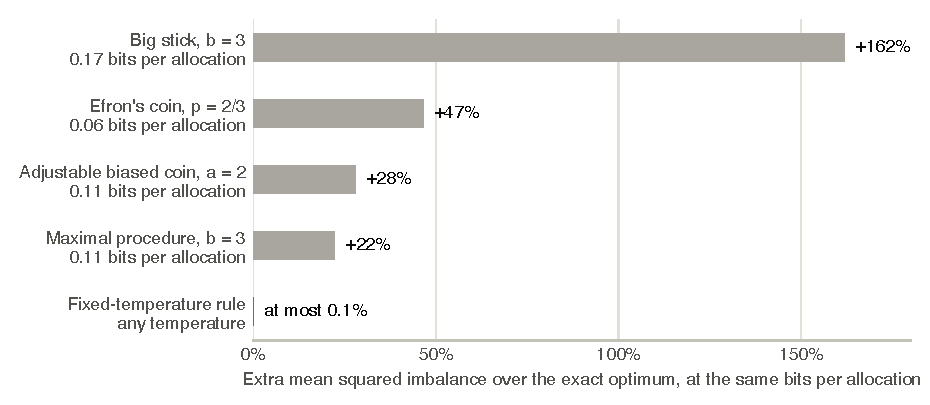
\includegraphics[width=\textwidth]{figures/fig2_twoarm.pdf}
\caption{Classical two-arm designs need 22--162\% more squared imbalance than the optimum at the same entropy rate; the fixed-temperature rule sits on the optimum. Excess mean squared imbalance against the exact KL-control optimum, at each design's usual setting. Across their parameter ranges the families stay above the optimum: Efron's coin by 6--65\%, the adjustable biased coin by 6--53\%, the maximal procedure by 17--27\% and the big stick by 77--431\%.}\label{fig:twoarm}
\end{figure}

%======================================================================
\section{Simulation study}\label{sec:sims}

With a budget of 1 bit per participant, exposure stayed within about one showing of target for all 1,000 participants, while complete randomization drifted to a standard deviation of 8.4. The same budget tolerated simultaneous enrollment and, with a ledger of completions, corrected the unequal condition representation that differential attrition caused under complete randomization.

\paragraph{Design.} We simulated the 64-vignette design of Section~\ref{sec:problem} under budgets from 0.25 to 8 bits, complete randomization (0 bits) and deterministic minimisation with random tie-breaking. Each run enrolled 1,000 participants, and each condition was replicated 10 times (6 times in the delay study, 8 in the attrition study). Exposure SD is averaged over participants 100 to 1,000 unless stated.

\subsection{Balance versus budget}

\paragraph{Any positive budget stops the drift.} Under complete randomization the SD grew from 2.6 after 100 participants to 8.4 after 1,000, when the most- and least-shown vignettes differed by 42 showings. With 1 bit it stayed between 0.9 and 1.0 throughout, and the final range was 4.4 showings (Figure~\ref{fig:traj}).

\begin{figure}[t]
\centering
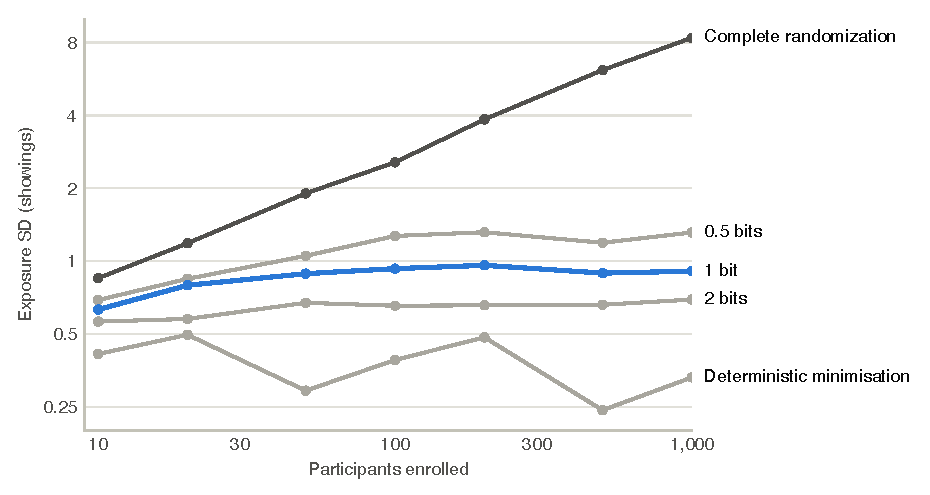
\includegraphics[width=\textwidth]{figures/fig3_trajectories.pdf}
\caption{Randomization drifts like $\sqrt{n}$; 1 bit per participant holds exposure SD near 0.9. Exposure SD after each number of participants, mean of 10 runs, both axes on log scales.}\label{fig:traj}
\end{figure}

\paragraph{Returns diminish quickly.} Each doubling of the budget cut the SD by roughly 30\%, so the SD scales about as $1/\sqrt{\kappa}$ (Figure~\ref{fig:budget}). Deterministic minimisation reached 0.40, near the floor that integer counts allow, while giving up 6.4 bits per participant on average.

\begin{figure}[t]
\centering
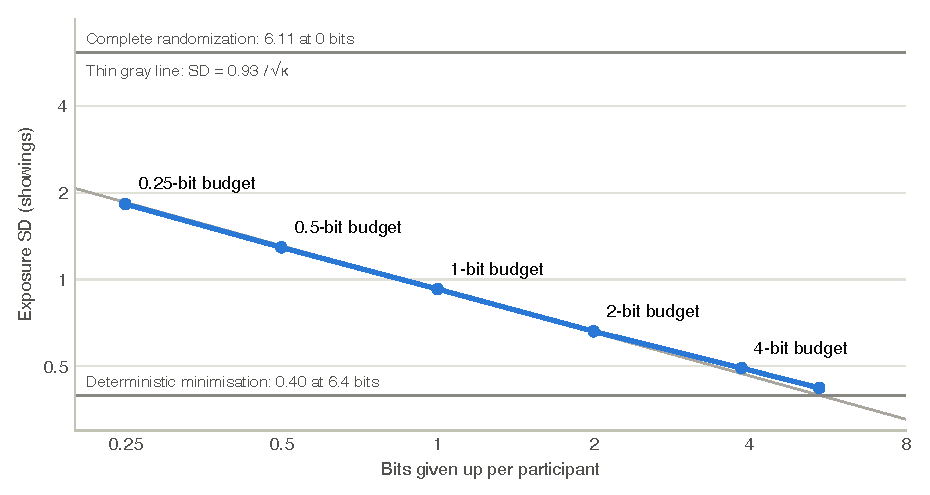
\includegraphics[width=\textwidth]{figures/fig4_budget.pdf}
\caption{Each doubling of the budget cuts exposure SD by about 30\%, to a floor near 0.4. Mean exposure SD over participants 100--1,000 against bits actually spent. The 4- and 8-bit budgets plot at the bits they spent, 3.9 and 5.4, because ties left nothing more to gain.}\label{fig:budget}
\end{figure}

\paragraph{Large budgets often cannot be spent.} At 4 bits, 13\% of participants met ties that left less than the budget to gain; at 8 bits, 63\% did. Beyond about 2 bits the extra balance is small, while allocation probabilities become far more unequal (Section~\ref{sec:order}).

\subsection{Simultaneous enrollment}

\paragraph{Delay punishes high gain.} When $b$ participants share one stale ledger, deterministic minimisation went from an SD of 0.40 at $b=1$ to 3.8 at $b=16$ and 17.7 at $b=64$, nearly three times worse than complete randomization (Figure~\ref{fig:delay}). Stochastic budgets degraded gracefully: at 1 bit the SD went from 0.93 to 1.24 and 2.10.

\begin{figure}[t]
\centering
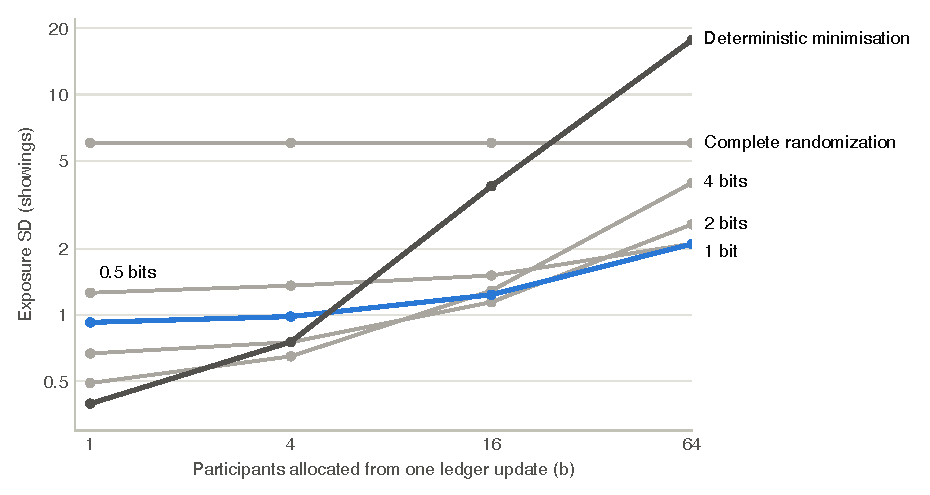
\includegraphics[width=\textwidth]{figures/fig5_delay.pdf}
\caption{When participants share a stale ledger, deterministic minimisation overshoots. Mean exposure SD over participants 100--960 when $b$ participants are allocated from one ledger update, 6 runs per condition, log scales. The ranking of budgets reverses as the delay grows: the classic trade-off between gain and delay in feedback control.}\label{fig:delay}
\end{figure}

\paragraph{The best budget shrinks as the delay grows.} With up to 16 simultaneous participants, 2 bits did best; with 64, budgets of 0.5 to 1 bit did. Counting participants as soon as they are assigned shortens the delay and is the first remedy (Section~\ref{sec:recs}).

\subsection{Differential attrition}

\paragraph{Counting completions restores equal representation of conditions; counting assignments does not.} Each participant dropped out with probability 15\% plus 6 points per vignette in their deck with factor A at its higher level, so dropout ranged from 15\% to 45\% and averaged about 30\%. Under complete randomization, factor A made up 48.4\% of completed showings instead of 50\%, and the exposure SD among completers reached 9.0 by 1,400 enrollments (Figure~\ref{fig:attrition}).

\begin{figure}[t]
\centering
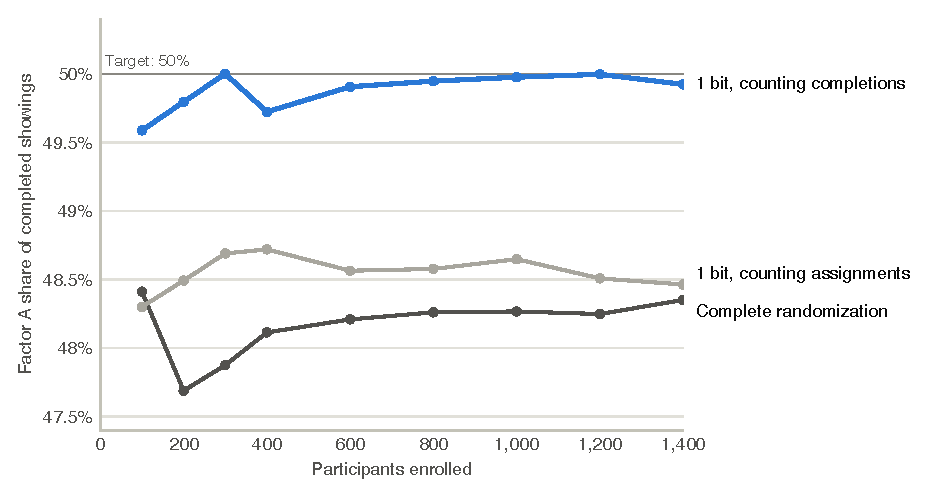
\includegraphics[width=\textwidth]{figures/fig6_attrition.pdf}
\caption{Only a ledger of completions keeps factor A at 50\% of completed showings. Share of completed showings with factor A at its higher level, mean of 8 runs; dropout 15--45\% by deck content. Deterministic minimisation with a ledger of completions also reached 50.0\%, with an exposure SD of 0.42 among completers.}\label{fig:attrition}
\end{figure}

\paragraph{The ledger decides what gets balanced.} With 1 bit and a ledger of assignments, assignments were balanced but completed data were not: factor A made up 48.5\% and the SD reached 5.3. With a ledger of completions, the same budget gave 49.9\% and an SD of 0.90, the same balance as with no attrition.

\paragraph{Equal counts do not make the estimates unbiased.} The simulation has no outcomes, so it shows which conditions completers saw, not who the completers are. When dropout depends on participants' characteristics, the completers in each condition can still differ, which is the selective attrition that \citet{zhou2016} documented, and the outcome analysis must still address it \citep{bell2013}.

\subsection{Order, factors and allocation probabilities}\label{sec:order}

\paragraph{Order stays balanced in expectation.} The G statistic for independence of vignette and position, divided by its degrees of freedom, lay between 0.98 and 1.06 for every budget, where 1 is what random order gives. Rolling one die for every slot shuffles the order, so no budget distorts it.

\paragraph{Factor levels are balanced too.} After 1,000 participants (5,000 showings), the worst of the six factors showed one level 103 more times than the other under complete randomization. At 1 bit the worst gap was 10, and under deterministic minimisation 3.

\paragraph{The price is unequal allocation probabilities at any moment.} After 500 participants at 1 bit, the most-favored vignette was 2.8 times as likely to be in the next deck as under complete randomization, and the least-favored 0.23 times as likely. These probabilities change with every participant, which is why the implementation logs them (Section~\ref{sec:recs}).

\subsection{Per-participant budget or fixed temperature}\label{sec:mode}

\paragraph{In this design the two versions behave alike.} We ran fixed temperatures, then per-participant budgets equal to the bits each temperature spent on average (Table~\ref{tab:mode}). With 64 stimuli the spread of deck totals is stable, so under a fixed budget $\beta$ barely moves: at 1 bit it stayed between 0.53 and 0.73 for 80\% of participants.

\begin{table}[ht]
\centering\small
\caption{Exposure SD under a fixed temperature and under a per-participant budget that spends the same bits on average (6 runs each, 600 participants).}\label{tab:mode}
\begin{tabular}{@{}cccc@{}}
\toprule
Fixed $\beta$ & Bits spent on average & SD, fixed $\beta$ & SD, per-participant budget \\
\midrule
0.3 & 0.49 & 1.29 & 1.31 \\
0.6 & 0.96 & 0.93 & 0.92 \\
1.2 & 1.90 & 0.68 & 0.67 \\
\bottomrule
\end{tabular}
\end{table}

\subsection{Runtime}

One allocation took 8--10 ms in Node.js on a laptop, and about 18 ms at the start of a study, when every deck ties. Building the list of admissible decks took 107 ms and 13 MB of memory.

%======================================================================
\section{Practical recommendations}\label{sec:recs}

Use a budget of 1 to 2 bits per participant, count participants when they are assigned and release them if they drop out, log every allocation probability, and state the budget in the protocol.

\paragraph{Choosing the budget.} The figures in Section~\ref{sec:sims} refer to the 64-vignette example; the ordering of the recommendations carries over to other designs (Table~\ref{tab:recs}). For a single treatment per participant the scale is different, because one allocation among two arms carries at most 1 bit. Efron's $p=2/3$ corresponds to 0.08 bits, so budgets for two-arm trials sit well below 1 bit.

\begin{table}[ht]
\centering\small
\caption{Choosing the budget.}\label{tab:recs}
\begin{tabularx}{\textwidth}{@{}XlX@{}}
\toprule
Situation & Budget per participant & Reason \\
\midrule
Default: participants enroll one at a time & 1 bit & Exposure SD about 0.9; each allocation as random as a uniform draw from half the admissible sets \\
Balance is paramount and enrollment is rarely simultaneous & 2 bits & Exposure SD about 0.66; little gain beyond this \\
Tens of participants can share one stale ledger & 0.5 to 1 bit & Lower gain overshoots less under delay \\
Staff who recruit could see the counts & as low as balance allows & The history reveals at most $\kappa$ bits about the next allocation \\
\bottomrule
\end{tabularx}
\end{table}

\paragraph{When a participant counts.} A ledger of assignments is fast but lets differential attrition skew which conditions completers saw, while a ledger of completions keeps completed showings balanced but reacts later. The better rule counts a participant at assignment and releases the count if they drop out or time out, as psiTurk does for sessions in progress \citep{gureckis2016}. Define ``completion'' in the protocol, including any exclusions such as failed attention checks.

\paragraph{Report attrition by condition.} Balanced completed showings do not make completers comparable across conditions, so report dropout by condition and analyze attrition as in any trial \citep{bell2013}.

\paragraph{Run it where nobody can see the ledger.} Compute allocations on a server and send each participant only their own conditions. This is the analogue of allocation concealment in trials \citep{schulz2002}, and it also prevents participants from reverse-engineering the design.

\paragraph{Log what the analysis will need.} For each participant, store the deck, its order, $\beta$, the log probability of the set, the budget, the code version and the random seed. These make the allocation auditable and support inverse-probability weighting \citep{horvitz1952} or randomization tests that replay the algorithm \citep{rosenberger2016}. Model-based analyses with participant and stimulus effects remain valid, because no allocation depends on that participant's own characteristics.

\paragraph{Report the allocation as a randomization method.} State the admissibility rule, the budget in bits, the ledger policy and its timeout, and how ties were broken, as CONSORT 2025 (item 17b) and SPIRIT 2025 (item 21b) ask for minimisation, including whether a random element was used \citep{hopewell2025,hrobjartsson2025}. Because every allocation keeps a stated random element, the method meets the ICH E9 call for a random element in every dynamic allocation \citep{ich1998} and the EMA instruction that deterministic schemes be avoided \citep{ema2015}. The budget makes that random element a number a reviewer can check.

%======================================================================
\section{Discussion}\label{sec:discussion}

Minimisation for sets of conditions is a feedback controller whose one natural parameter is entropy. Most of its ingredients have precedents; what is new is applying them to constrained sets of conditions, enrolled online, with a budget that can be reported and checked.

\paragraph{Single-treatment allocation.} \citet{klotz1978} derived exponential allocation probabilities by maximizing entropy under a balance constraint, re-solved for each patient, and \citet{ryeznik2018} extended the rule to several arms with one parameter. The biased coins of \citet{smith1984} and \citet{ball1993} are fixed-temperature rules of the same kind, and Wei's (\citeyear{wei1977}) urn is, asymptotically, the unit-temperature rule on the ledger's Jensen--Shannon gain. We make the entropy budget itself the parameter, show what a per-allocation budget costs when there are few arms, and give the exact control identity.

\paragraph{Online and combinatorial balancing.} Herding \citep{welling2009,chen2016} and the self-balancing walk \citep{alweiss2021}, which \citet{arbour2022} adapted to online experiments, balance running sums with deterministic or randomized feedback. The Gram--Schmidt walk design trades robustness against balance with one parameter \citep{harshaw2024}, and best-of-$K$ rerandomization bounds the loss of robustness through $\log K$ \citep{banerjee2020}. None of these allocates constrained sets per participant, and the best-of-$K$ bound says nothing once the $K$ draws are repeated for every participant; a per-participant entropy budget is the natural replacement.

\paragraph{Stale counts in trials.} We found no prior analysis of minimisation when several sites allocate from the same out-of-date counts. Emergency trials sidestep the delay by computing each site's next allocation in advance \citep{zhao2010}, and response-adaptive designs have been analyzed under delayed responses \citep{bai2002}. Our delay results also bear on Taves's (\citeyear{taves2010}) view that a random element is rarely needed: under simultaneous enrollment, removing it made minimisation worse than randomization.

\paragraph{Vignette, conjoint and choice designs.} Standard practice builds decks offline, for instance with D-efficient or confounded factorial designs, and then randomizes their order \citep{atzmuller2010,dulmer2016,su2020}. The two approaches combine naturally: an offline design's decks can serve as the admissible set, and the allocator then balances how often each deck is used as participants arrive.

\paragraph{Limitations.}
\begin{enumerate}
\item Shannon entropy is not predictability. With two arms and an imbalance bound of 3, the maximal procedure has more entropy than the big stick (0.89 against 0.83 bits per allocation) but is easier to guess (0.625 against 0.583). Where guessing matters, report a guessing measure as well.
\item The ledger here counts conditions only. Balancing participants' covariates, positions or pairs of conditions needs a richer ledger; any cost that is linear in counts keeps the dice, but weighted costs need re-weighted dice to stay optimal.
\item Exact calibration needs the admissible sets enumerated. Larger designs need Monte Carlo calibration, whose accuracy we have not studied systematically.
\item Plain rejection stalls at very low temperatures, so the implementation falls back to drawing from the enumerated list.
\item The simulations cover one design. The $1/\sqrt{\kappa}$ scaling and the delay results should be checked in others.
\item Allocation probabilities vary from participant to participant. Design-based estimators should use the logged probabilities, and inference for within-participant effects under this design deserves its own treatment.
\item Balanced completed showings are not unbiased estimates. The attrition study shows only that the method corrects unequal condition representation caused by differential attrition; it simulates no outcomes, and when dropout depends on participants' characteristics the completers in each condition can still differ \citep{zhou2016}.
\end{enumerate}

\paragraph{Future work.} Three directions follow. One is robustness bounds indexed by the per-participant budget; another is non-uniform targets and covariate-adaptive ledgers. The third is ledgers that predict in-progress sessions across sites, which would shorten the effective delay.

\paragraph{Code availability.} The implementation and the simulation scripts are at \url{https://github.com/andrewbistras/min_sim}, in the \texttt{paper/} folder, and reproduce every number and figure in this paper. Running \texttt{sh run\_all.sh} in \texttt{paper/sim} reruns all of them.

%======================================================================
\appendix
\section{Proofs}\label{app:proofs}

Throughout, $E(S)=\sum_{i\in S}c_i$ is a deck's total count, $\Unif$ is the uniform law on $\A$, and $\pi_\beta(S)\propto\exp(-\beta E(S))$.

\paragraph{Proposition~\ref{prop:maxent}.} For any law $\pi$ on $\A$, expanding $\KL(\pi\,\|\,\pi_\beta)\ge 0$ gives
\[
\KL(\pi\,\|\,\Unif) + \beta\,\E_\pi[E] \;\ge\; -\log\E_{\Unif}\big[e^{-\beta E}\big] \;=\; \KL(\pi_\beta\,\|\,\Unif) + \beta\,\E_{\pi_\beta}[E].
\]
So any $\pi$ that spends no more bits than $\pi_\beta$ has an expected total count at least as large, for $\beta>0$. \qed

\paragraph{Proposition~\ref{prop:dice}.} Every ordered roll of an admissible set $S$ has probability $\prod_{i\in S}\tilde w_i$, which is proportional to $\exp(-\beta E(S))$ and so depends on the set alone. Conditioning on admissibility therefore gives the set law $\pi_\beta$ and makes all $k!$ orders equally likely. \qed

\paragraph{Proposition~\ref{prop:js}.} Adding deck $S$ gives counts $c+x(S)$ over $k(t+1)$ showings, so $P_{t+1}=wP_t+(1-w)U_S$ with $w=t/(t+1)$.
(a) In $\JS_w$ only $H(P_{t+1})$ depends on $S$.
(b) Expanding $H(u+\delta)=\log m-\frac{m}{2}\|\delta\|^2+O(\|\delta\|^3)$ around the uniform $u$, and using $\sum_i(c_i+x_i-T)^2=\text{const}+2E(S)$ with $T=k(t+1)/m$, gives $\JS_w=\text{const}-mE(S)/(kt+k)^2$.
(c) $P_t$ is the equal-weight mixture of $U_{S_1},\dots,U_{S_t}$, each with entropy $\log k$.
(d) Let $\mathcal{H}$ be the history, $\pi_{\mathcal{H}}$ the law of the next set and $\bar\pi$ its average over histories. Then $\E[\KL(\pi_{\mathcal{H}}\,\|\,\Unif)]=I(\mathcal{H};S)+\KL(\bar\pi\,\|\,\Unif)\ge I(\mathcal{H};S)$, so a per-participant budget $\kappa$ bounds $I(\mathcal{H};S)$ by $\kappa$. \qed

\paragraph{Proposition~\ref{prop:control}.} The Bellman equation of the average-cost problem \citep{todorov2009} is $c+v(e)=q(e)-\log\E_{\Unif}[\exp(-v(e'))]$, with optimal policy $\pi^*(S\mid e)\propto\exp(-v(e'))$. With $v(e)=\frac{\beta}{2}\|e\|^2$ and $\sum_i e_i=0$, the next value is $v(e')=v(e)+\beta\sum_{i\in S}e_i+\text{const}$, so $\pi^*=\pi_\beta$, and the equation holds for $q=q_\beta$ with the constants absorbed into $c$. With two arms and $D=n_A-n_B$ the surpluses are $\pm D/2$, and $\E_{\Unif}[\exp(-\beta e_S)]=\cosh(\beta D/2)$. \qed

\paragraph{Proposition~\ref{prop:stability}.} Let $V(e)=\|e\|^2$; then $\E[\Delta V\mid e]=2\,\E_\pi[X]+k(1-k/m)$, with $X=\sum_{i\in S}e_i$. We proceed in three steps.
\begin{enumerate}
\item \emph{A good deck always exists.} Under $\Unif$, $X$ has mean 0, because every stimulus lies in the same number of admissible sets. Its variance is at least $\lambda\|e\|^2$, and $X\le k\|e\|$. The Bhatia--Davis inequality then gives $\min_S X\le-(\lambda/k)\|e\|$.
\item \emph{Fixed $\beta$.} The Gibbs law lies within $\log|\A|/\beta$ of the minimum, so $\E[\Delta V]\le-2(\lambda/k)\|e\|+2\log|\A|/\beta+k$.
\item \emph{Budget $\kappa$.} The mixture $\varepsilon\,\delta_{S^*}+(1-\varepsilon)\Unif$ that spends $\kappa$ bits has $\E[X]=\varepsilon\min_S X$, and by Proposition~\ref{prop:maxent} the budgeted rule does at least as well. So $\E[\Delta V]\le-2\varepsilon(\lambda/k)\|e\|+k$, where $\varepsilon$ depends only on $\kappa$ and $|\A|$.
\end{enumerate}
In both cases the drift is negative outside a bounded set, and Foster's criterion gives positive recurrence and a finite long-run average of $\E\|e(t)\|$ \citep{meyn2009}. \qed

\section{Admissible decks in the \texorpdfstring{$2^6$}{2\^{}6} example}\label{app:decks}

The independent sets of the six-cube number 64, 1,824, 30,720, 342,400 and 2,682,432 for sizes 1 to 5. Of the admissible five-sets, 201,376 contain only vignettes with an even number of factors at their higher level, and 201,376 only odd ones; such single-parity sets satisfy the rule automatically.

Under complete randomization over admissible decks, two vignettes at Hamming distance 2 share a deck with probability 0.0060, against 0.0053 for distances 3 to 6. Context effects that depend on pairs should keep that 13\% difference in mind. The covariance of the inclusion vector has eigenvalues from 0.055 to 0.117 on the sum-zero subspace, so the stability constant of Proposition~\ref{prop:stability} is $\lambda=0.055$.

\section{Exact calibration by enumeration}\label{app:calib}

Enumerate $\A$ once. For each participant, tally the histogram $N_E$ of $E=\sum_{i\in S}(c_i-\min c)$ over $\A$, and evaluate $\kappa(\beta)$ from \eqref{eq:calib}. Bisect on $\beta$ until $\kappa(\beta)$ equals the budget.

If the budget is at least $\log(|\A|/N_{E_{\min}})$, set $\beta=\infty$ and draw uniformly among the minimum-total decks. For that draw, pick the $r$-th such deck in a second pass, with $r$ uniform. Both passes cost one sweep over $\A$ (about 5 ms in the example).

\section{The candidate-pool approximation}\label{app:pool}

A tempting implementation draws $M$ admissible decks uniformly and picks one with probabilities proportional to $\exp(\gamma\times\text{score})$. It is sampling-importance-resampling \citep{smithgelfand1992} aimed at $\pi_\beta$, and it has two knobs, $M$ and $\gamma$.

The two knobs are one. With a score that also counted positions (weight 0.075), pools of 10 to 1,000 decks and values of $\gamma$ from 0.05 to 1 all fell within about 2\% of the exact dice curve when indexed by bits spent. The entropy of the pool's softmax, $H_{\text{pool}}$, already measures the budget: $\ln M-H_{\text{pool}}$ was 0.39 nats where the true spend was 0.40.

Two add-ons behaved unexpectedly. A fixed bonus for chosen vignettes raised their counts by a constant of about 1.4 showings rather than by a proportion, 5.7\% after 320 participants but 0.5\% after 3,000. A small position term (weight 0.075) improved order balance by only about 8\% over shuffling the order.

\bibliographystyle{apalike}
\bibliography{refs}

\end{document}
